%!TEX root = ./intern_report.tex

\newpage
\subsection{Building Wallie: A Hardware Platform for Data Collection and Deployment}

\paragraph{}
The Robotics and Autonomous Systems Group of DATA61 is about field robotics. Therefore, it is not sufficient to demonstrate a concept theoretically or just by simulations. Instead, the members are expected to demonstrate our systems and results in complex real world environments.

\paragraph{}
Therefore, we needed a robot platform on which we can collect data and perform our tests. However, the available platforms of CSIRO were all in use for bigger projects. Hence we were requested to build a robot platform based on Pololu Wild Thumper chassis. This platform was previously assembled by our seniors: Isuru and Tharindu. However, as we describe below, we had to change almost every component of that to create a new robot to suit our specific needs. Our friend from Chile named this robot Wallie, in reference to the Wall-E movie and the fact our robot was initially built to follow walled hallways.

\begin{figure}[H]
    \centering
    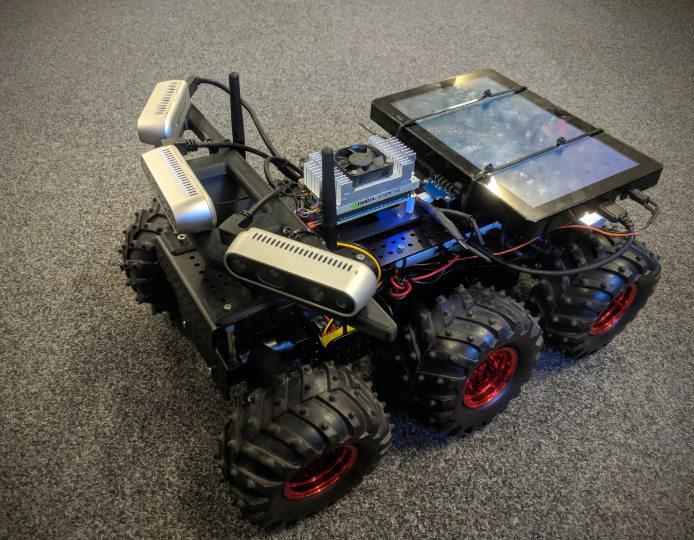
\includegraphics
        [width=10cm]
        {figures/wallie.PNG}
    \caption{Wallie: The Robot \label{Fig:wallie}}\vspace{-4mm}
\end{figure}

\paragraph{}
Firstly, we need a way to fix cameras in the robot for data collection and testing. I sketched a small camera rig to hold three Intel Realsense cameras, each facing: center, left and right at 30 degree angles from center. Samith Ashan, my coworker helped designed it in solidworks. That, a platform for the Jetson TX2 board and a holder for the Li-ion battery were then 3D printed. 

\subsubsection{Designing the Power Distribution System}

\begin{figure}[H]
    \centering
    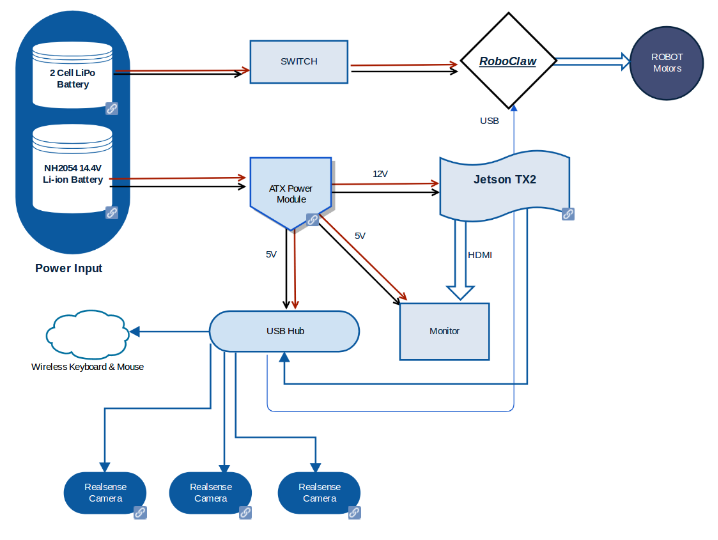
\includegraphics
        [width=13cm]
        {figures/wallie_hardware.PNG}
    \caption{Wallie: Hardware Hierarchy }\vspace{-4mm}
\end{figure}

\paragraph{}
We then designed a power distribution system for the robot, to deliver power from two batteries to all the sensors and actuators. We consulted Dr. Navinda and Mr. James Brett and came of with the following system. A 3 cell Li-Po delivers power to the Roboclaw Motor Controller, to which six 12V, 2.5D high torque motors are connected through a switch and a fuse (to prevent damage to the motor controller in case if the motors start stalling, as it happened once). The cameras and IMU are powered through an active USB hub. The USB hub LCD display and NVIDIA Jetson TX2 are powered through a robust power supply (12V, 5V) which is connected through a switch to the 7.4V Li-ion battery. Having two separate power sources for high-level and low-level systems helped through decoupling by reducing the chances of power failures from one network damaging the component in the other.

\paragraph{}
We documented the design of the robot in CSIRO's confluence wiki pages, so that fellow researchers can use it in the future for their own activities. Most of our time in CSIRO (about 75\%) was spent in building and debugging the robot platform. 


\subsubsection{NVIDIA Jetson TX2}

\paragraph{}
Jetson TX2 ~\cite{jetson_tx2} is device released by NVIDIA as a solution to run computation-intensive programs on board of a low power consuming device. This credit-card sized device contains CPU that can run AMD64 Linux, a powerful GPU that can run multiple neural networks at once using just 7.5W of power. DATA61 RAG is starting to unify and standardize their sensor and actuator APIs. Hence, they were considering NVIDIA's Jetson TX2 and Xavier as potential candidates for the high level controller on their multiple types of wheeled, legged and aerial robots.



% Table: Jetson
\begin{table}[H]
    \begin{center}
        \caption {NVIDIA Jetson TX2 Specifications} \label{tab:jetson}
        \begin{tabular}{|| r || l ||}    
            \hline
            GPU             & 256 CUDA cores of Pascal Architecture \\
            \hline
            CPU             & HMP Dual Denver 2/2 MB L2 + Quad ARM® A57/2 MB L2 \\
            \hline
            Memory          & 8 GB 128 bit LPDDR4, 59.7 GB/s \\
            \hline
            Data storage    & 32 GB \\
            \hline 
            USB             & USB 3.0 \\
            \hline 
            Connectivity    & Gigabit Ethernet, 802.11ac WLAN, Bluetooth \\
            \hline   
        \end{tabular}    
    \end{center}
\end{table}

\paragraph{}
Hence we began using Jetson TX2 ~\cite{jetson_tx2} as the high level controller with Orbitty carrier board. We flashed it with NVIDIA's Linux for Tegra kernel and set it up with Jetpack 3.2.1 (Updated to Jetpack 3.3 later).

% Image: Jetson
\begin{figure}[H]
    \centering
    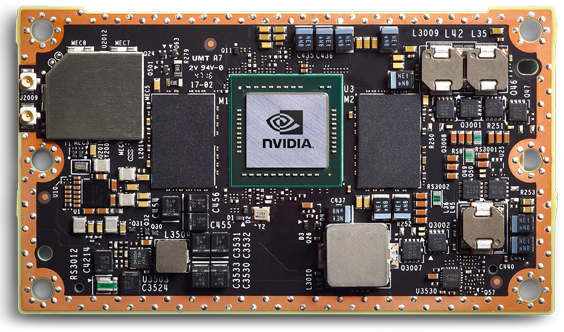
\includegraphics
        [width=8cm]
        {figures/jetson.png}
    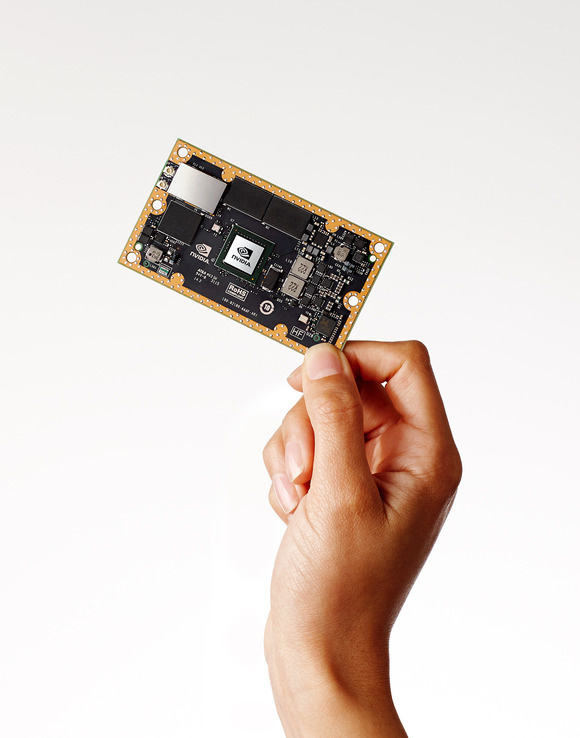
\includegraphics
        [height=5cm]
        {figures/jetson_scale.jpg}
    \caption{NVIDIA Jetson TX2 }\vspace{-4mm}
\end{figure}


\newpage
\subsubsection{Intel Realsense Depth Camera D435}

% Image: Realsense
\begin{figure}[H]
    \centering
    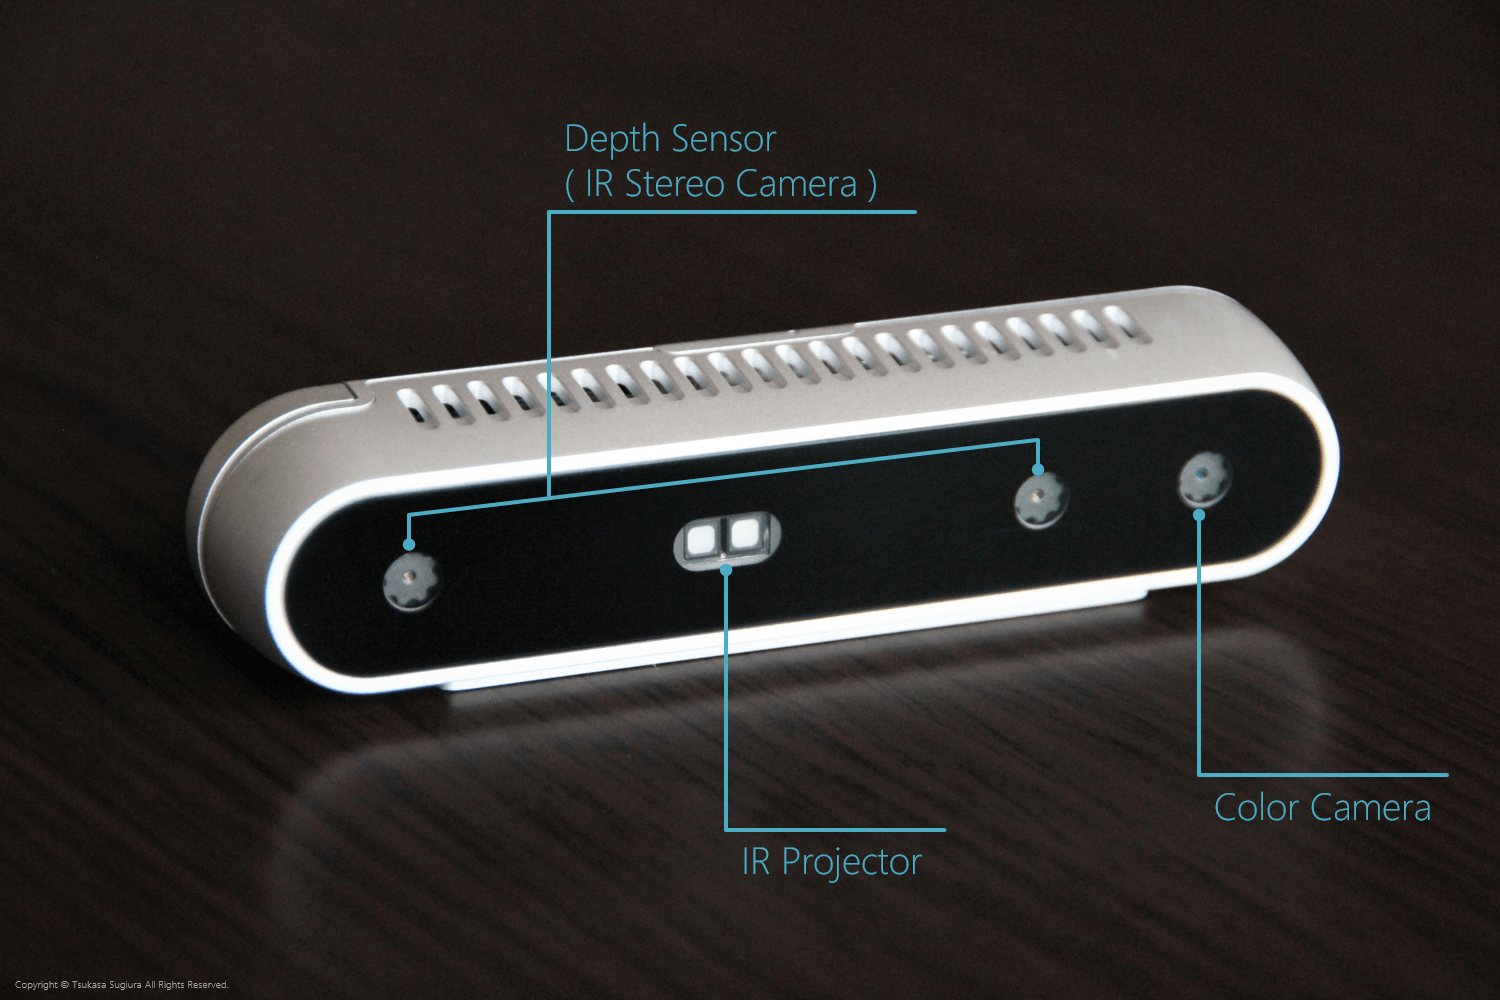
\includegraphics
        [width=8cm]
        {figures/realsense.png}
    \caption{Intel Realsense D435}\vspace{-4mm}
\end{figure}

\paragraph{}
Intel Realsense depth camera is able to output image streams of RGB, IR and Depth images as per following specifications. Due to the small size and versatility, RAG members considered using this as he de-facto vision sensor in low power robots. It can be connected to Jetson TX2 via a USB-C cable and there is an official ROS package from Intel with which it can communicate via serial and publish the image streams and diagnostic information.

% Table: Realsense
\begin{table}[H]
    \begin{center}
        \caption {Intel Realsense D435 Specifications} \label{tab:realsense}
        \begin{tabular}{|| r || l ||}
            \hline
            Depth FOV (Horz, Vert, Diag)	& 85.2\degree x 58\degree x 94\degree (+/- 3\degree) \\
            \hline
            Depth Stream Output Resolution	& Up to 1280 x 720 \\
            \hline
            Depth Stream Output Frame Rate	& Up to 90 fps \\
            \hline
            Maximum Range	                & Approx.10 meters \\
            \hline
            RGB   FOV (Horz, Vert, Diag)	& 69.4\degree x 42.5\degree x 77\degree (+/- 3\degree) \\
            \hline
            RGB   FOV (Horz, Vert, Diag)	& 1920 x 1080 at 30 fps \\
            \hline
            Connectors	                    & USB 3.0 Type - C \\
            \hline
        \end{tabular}    
    \end{center}
\end{table}

\paragraph{}
We used three of these cameras, each facing 30\degree left, right and center to collect image streams in ROSbags. We used RGB image stream to train our network, since most other robots do not have depth cameras as vision sensors. The depth data we collected was used by our coworker along with our IMU data for SLAM purposes.

\subsubsection{Roboclaw Motor Controller}

\paragraph{}
The wild thumper chassis we obtained had the arduino-based TREX motor controller on it. I spent few days trying to come up with an algorithm that can map the remote-control pulses to the PWM commands for smooth maneuvering. I succeeded partially. However, due to the problems described in the next section, we switched to Roboclaw controller, which mixes RC pulses into PWM using their proprietary algorithm.  

% Table: Roboclaw
\begin{table}[H]
    \begin{center}
        \caption {Pololu Roboclaw Motor Controller Specifications} \label{tab:roboclaw}
        \begin{tabular}{|| r || l ||}    
            \hline
            Motor channels              &   2   \\
            \hline
            Control interface           &	USB; TTL serial (2-way), RC pulses; PWM\\
            \hline
            Minimum operating voltage   &	6 V \\
            \hline
            Maximum operating voltage   &	34 V \\
            \hline
            Continuous output current per channel   &	30 A \\
            \hline
            Peak output current per channel         &	60 A \\
            \hline   
        \end{tabular}    
    \end{center}
\end{table}

\paragraph{}
The main advantage for choosing roboclaw was the availability of a compatible ROS package. However, we then found that the package was not being maintained for the past few years. I spent multiple weeks debugging the package and rewriting some of the driver code.

% Image: 2 motor controllers
\begin{figure}[H]
    \centering
    \begin{minipage}{.5\textwidth}
        \centering
        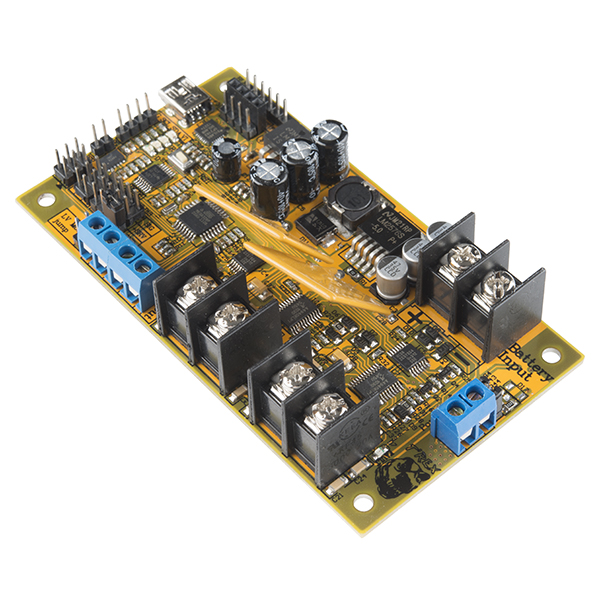
\includegraphics[width=0.8\linewidth]{figures/trex.jpg}
        \captionof{figure}{TREX Motor Controller}
        \label{fig:test1}
    \end{minipage}%
    \begin{minipage}{.5\textwidth}
        \centering
        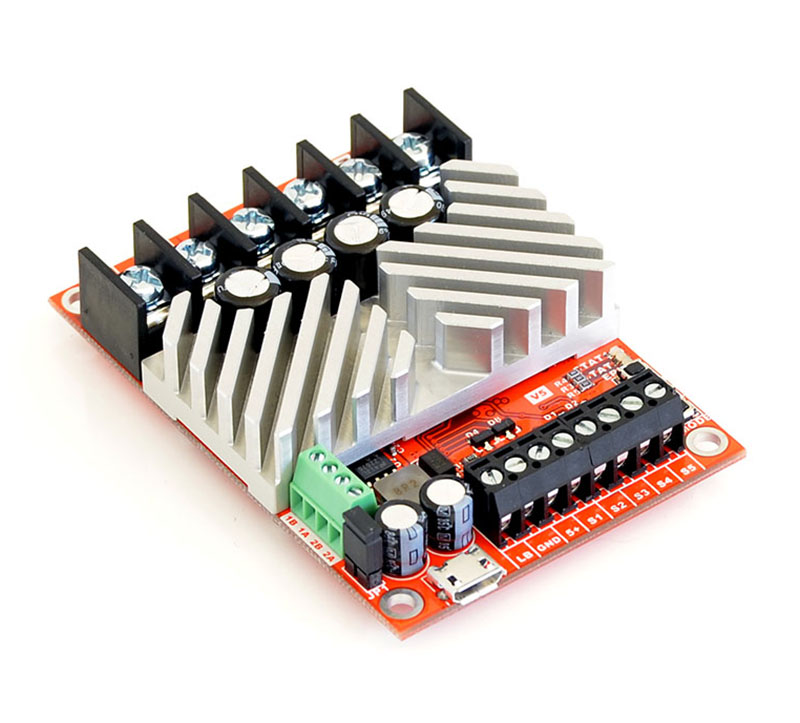
\includegraphics[width=0.8\linewidth]{figures/roboclaw.jpg}
        \captionof{figure}{Roboclaw Motor Controller}
        \label{fig:test1}
    \end{minipage}
\end{figure}

\subsubsection{Lord Microstrain IMU}

% Image: Realsense
\begin{figure}[H]
    \centering
    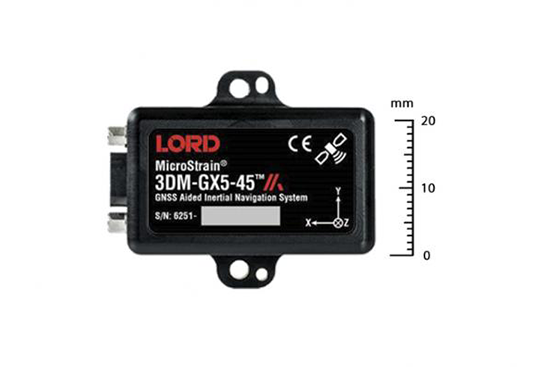
\includegraphics
        [width=8cm]
        {figures/imu.png}
    \caption{Lord Microstrain 3DM®-GX5-45 GNSS-Aided Inertial Navigation System}\vspace{-4mm}
\end{figure}

\paragraph{}
Lord Microstrain 3DM®-GX5-45 GNSS-Aided Inertial Navigation System is the state of the art IMU sensor. We were given one of these to be used as the IMU sensor in our robot for hill-climbing. We found a relevant ROS package that can interface with the device via serial and publish the readings in two forms: rotation quaternions and cartesian vector components of the perceived acceleration. I used the vector components to find the direction of the slope.\\



\begin{table}[H]
    \begin{center}
        \begin{tabular}{|| r || p{10cm} ||}
            \hline
            Integrated sensors             	& Triaxial accelerometer, triaxial gyroscope, triaxial magnetometer, pressure altimeter,temperature sensors, GNSS \\
            \hline
            IMU Outputs                 	& acceleration, angular rate, magnetic field , ambient pressure, deltaTheta, deltaVelocity\\
            \hline
        \end{tabular}   
        \newline
        \caption {Lord Microstrain 3DM®-GX5-45 GNSS-Aided Inertial Navigation System Specifications} \label{tab:realsense}
        
        \begin{tabular}{|| r || l || l || l ||}
            \hline
            Metric          & Accelerometer & Gyroscope & Magnetometer \\
            \hline
            std. range      & +/- 8 g       & +/- 300\degree/sec  & +/- 2.5 Gauss \\
            \hline
            Non linearity   & +/- 0.02 \% fs   & +/- 0.02 \% fs      & +/- 0.3 \% fs \\
            \hline
            Resolution      &<0.1 mg        &    <0.003\degree/sec &           --\\
            \hline
           
        \end{tabular}
        
    \end{center}
\end{table}


\newpage
\subsubsection{Problems Faced and Solutions}

\paragraph{}
Firstly, when we assembled wallie with TREX as the low level controller and a custom algorithm to mix RC signals into PWM values for motor control, we found that it was quite difficult to maneuver the robot. Using remote control, we could not make it take tight turns at corners and the robot did not turn smoothly in carpeted floors due to friction. We found three problems that resulted in this:

\begin{itemize}
    \item Center of mass of the assembled robot was not exactly at the geometric center.
    \item RC mixing algorithm was not robust enough
    \item The MOSFET switch used between the battery and TREX limits the current, reducing the torque of motors.
\end{itemize} 

\paragraph{}
To solve these issues, I improved the mixing algorithm, Uvindu reassembled the robot and we removed the switch. The performance improved, but after few hours of test run, the TREX controller burnt off. Dr. Navinda instructed us to troubleshoot it and submit a report. After intensive testing and discussion with James Brett, Pubudu Aravinda and Samith Ashan, we identified the key issue as the in-built fuses of the old TREX board that failed to function as a large current was drawn when motors stalled on the rough carpet floor. As a result, the hall sensor on the controller got burnt, short circuiting and damaging two MOSFETs on the same side of the H-bridge. Dr. Navinda accepted the report and ordered the Roboclaw controller as replacement (since TREX boards are outdated and unavailable in the market). 

\paragraph{}
The prime advantage of the new Roboclaw was the associated ROS package. However, we soon found that the public package was severely outdated and not maintained. I contacted the manufacturers of Roboclaw and got a copy of the ROS package they use internally. That package also had several issues which we struggled with, throughout the project. After a week of debugging, I realized a main issue was that their driver was not thread safe. That is, when the ROS node receives a message, it runs the specified callback function, which is initiated on a new thread. If multiple such function calls are made in quick succession, it results in multiple threads that try to access the same resources (serial port). This results in unexpected frequent crashes. I changed the driver package to be thread safe and fixed some issues with incompatibility between velocity commands and odometry readings.

\paragraph{}
The D435 Realsense cameras are also not error free. We noticed that their output serial stream hangs unexpectedly and the only known solution is to unplug and plug them back. After some reading, I found that this is a hardware bug addressed by Intel as unfixable on this device. Therefore, I recommended Nick to not rely on these devices for critical tasks, such as the DARPA subterranean challenge.

\paragraph{}
When collecting data for hill climbing, I noticed a large variance (noise) in the IMU readings. Since our neural networks consider only the current inputs to provide instantaneous output velocity, noise in such an input would hinder the training process as the optimizer struggles to find correlation. I noticed that this high variance was due to the small slope of the hills and the increase in the percentage error due to that. To avoid this, I suggested fixing the IMU at an elevated angle to the horizontal on the robot.

\paragraph{}
We also faced issues with Jetson TX2, since the orbitty development board which we had to use (due to its small form factor) had its own modified Linux kernel. Many drivers were not directly supported for this and we had to modify the kernel to install certain drivers.